% This file was created with tikzplotlib v0.10.1.
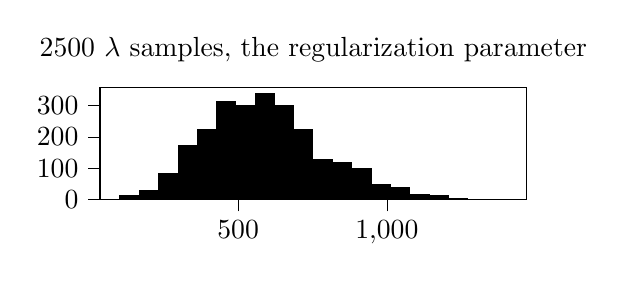
\begin{tikzpicture}

\definecolor{darkgray176}{RGB}{176,176,176}

\begin{axis}[
height=3cm,
tick align=outside,
tick pos=left,
title={2500 \(\displaystyle \lambda\) samples, the regularization parameter},
width=7cm,
x grid style={darkgray176},
xmin=35.7279701210218, xmax=1469.98795606424,
xtick style={color=black},
y grid style={darkgray176},
ymin=0, ymax=357,
ytick style={color=black}
]
\draw[draw=none,fill=black] (axis cs:100.921605845714,0) rectangle (axis cs:166.115241570406,16);
\draw[draw=none,fill=black] (axis cs:166.115241570406,0) rectangle (axis cs:231.308877295097,32);
\draw[draw=none,fill=black] (axis cs:231.308877295098,0) rectangle (axis cs:296.502513019789,86);
\draw[draw=none,fill=black] (axis cs:296.502513019789,0) rectangle (axis cs:361.696148744481,173);
\draw[draw=none,fill=black] (axis cs:361.696148744481,0) rectangle (axis cs:426.889784469173,227);
\draw[draw=none,fill=black] (axis cs:426.889784469173,0) rectangle (axis cs:492.083420193865,315);
\draw[draw=none,fill=black] (axis cs:492.083420193865,0) rectangle (axis cs:557.277055918557,303);
\draw[draw=none,fill=black] (axis cs:557.277055918557,0) rectangle (axis cs:622.470691643249,340);
\draw[draw=none,fill=black] (axis cs:622.470691643249,0) rectangle (axis cs:687.664327367941,302);
\draw[draw=none,fill=black] (axis cs:687.664327367941,0) rectangle (axis cs:752.857963092633,224);
\draw[draw=none,fill=black] (axis cs:752.857963092633,0) rectangle (axis cs:818.051598817325,129);
\draw[draw=none,fill=black] (axis cs:818.051598817325,0) rectangle (axis cs:883.245234542017,120);
\draw[draw=none,fill=black] (axis cs:883.245234542017,0) rectangle (axis cs:948.438870266709,100);
\draw[draw=none,fill=black] (axis cs:948.438870266709,0) rectangle (axis cs:1013.6325059914,51);
\draw[draw=none,fill=black] (axis cs:1013.6325059914,0) rectangle (axis cs:1078.82614171609,41);
\draw[draw=none,fill=black] (axis cs:1078.82614171609,0) rectangle (axis cs:1144.01977744078,17);
\draw[draw=none,fill=black] (axis cs:1144.01977744078,0) rectangle (axis cs:1209.21341316548,15);
\draw[draw=none,fill=black] (axis cs:1209.21341316548,0) rectangle (axis cs:1274.40704889017,5);
\draw[draw=none,fill=black] (axis cs:1274.40704889017,0) rectangle (axis cs:1339.60068461486,3);
\draw[draw=none,fill=black] (axis cs:1339.60068461486,0) rectangle (axis cs:1404.79432033955,1);
\end{axis}

\end{tikzpicture}
